%\todo{2S - сюда нужно вставить переведенные текст с картинками materials\/cosb\_2019\/paper\_rev\_v10.docx, картинки нужно засунуть в гугл Draw (папка p2) - там перевести наложив поверх английского текста русский. Ссылки на литературу уже загружены в зотеро. Все заголовки начинать с уровня subsection и далее}


% \section{Реферат}

%     Нуклеосомы являются фундаментальными единицами уплотнения хроматина, которые обертывают около $\sim$ 150 пар оснований ДНК вокруг октамера гистоновых белков. Их повсеместное присутствие в ядре клетки с тех пор, как первые эукариоты заставили хроматиновый аппарат совместно развиваться и научиться использовать различные способы динамики нуклеосом и ощущать различия в составе нуклеосом. Изменения последовательностей гистонов или ДНК, посттрансляционные модификации (PTM) гистонов, рекрутирование белков хроматина модулируют динамику нуклеосом и обеспечивают эпигенетическую регуляцию путей обработки ДНК (транскрипция, репликация, репарация и т. Д.). Наше понимание этого сложного взаимодействия между составом, динамикой и функционированием нуклеосом постоянно развивается благодаря новым знаниям и открытиям. В этом обзоре мы выделяем последние достижения в этой области, пытаясь организовать их в единую структуру.

% \subsection{Введение}

    Жизнь эукариотических клеток полностью управляется пространственно-временной организацией хроматина внутри ядер клеток. Хроматин не только компактизует ДНК, но и служит средой для расшифровки и интерпретации генетической информации \cite{van_holde_chromatin_1989}. Основной структурной единицей организации хроматина является нуклеосома - повторяющаяся единица из примерно 200 пар оснований ДНК, организованная гистоновыми белками \cite{olins_spheroid_1974,kornberg_chromatin_1974-1} (Рис. \ref{fig:part2_1_f1}a). Центральные 145–147 пар оснований ДНК образуют коровую частицу нуклеосомы, или нуклеосомный кор (NCP, nucleosome core particle), плотно наматываясь на октамер гистонов в виде $\sim$1,7 витка левой суперспирали \cite{luger_crystal_1997,tan_nucleosome_2011}. Линкерные сегменты ДНК фланкируют NCP. Канонический октамер гистонов состоит из двух пар идентичных гистоновых димеров H3-H4 и H2A-H2B, образованных коровыми гистонами H3, H4, H2A и H2B, соответственно (Рис. \ref{fig:part2_1_f1}a) \cite{draizen_histonedb_2016}. Симметрия октамера наделяет NCP осью псевдосимметрии второго порядка, которая определяет расположение центра ДНК - диады нуклеосом. Все четыре типа гистонов, вероятно, имеют общее эволюционное происхождение и имеют сходную структуру  \cite{malik_phylogenomics_2003,bhattacharyya_archaeal_2018} (Рис. \ref{fig:part2_1_f1}б). Гистоны также подразделяются на основные ``канонические'' гистоны (депонируются на ДНК при репликации) и альтернативные варианты гистонов, которые синтезируются в течение клеточного цикла и могут быть тканеспецифичными \cite{draizen_histonedb_2016}. Дополнительные уровни вариабельности нуклеосом обеспечиваются репертуаром посттрансляционных модификаций гистонов (ПТМ) \cite{bowman_post-translational_2015} и вариаций внутри последовательностей ДНК (Рис. \ref{fig:part2_1_f1}в).

С годами стало ясно, что нуклеосомы претерпевают множество функционально важных структурных и динамических перестроек во время всех ключевых процессов происходящих в хроматине (транскрипция, репликация, репарация ДНК и т.д.) \cite{zlatanova_nucleosome_2009,chen_asymmetric_2017}. Более того, способность нуклеосом претерпевать определенные типы конформационных переходов разумно используется многими белками хроматина, включая ремоделирующие хроматин \cite{sinha_distortion_2017,liu_mechanism_2017,ranjan_h2a_2015-1}, факторы транскрипции \cite{laptenko_p53_2011,zaret_pioneer_2016}, шапероны \cite{valieva_large-scale_2016}, РНК-полимеразы \cite{gaykalova_structural_2015} и т.д. С момента появления первых эукариот около 2 миллиардов лет назад биологические процессы ядра приспосабливались к структуре нуклеосомы, используя тонкие детали ее динамики. Одновременно с диверсификацией репертуара нуклеосом с помощью вариантов гистонов и их ПТМ белки хроматина также диверсифицировались и эволюционировали, чтобы различать разные нуклеосомы по их структурным и динамическим характеристикам. Это тонкое взаимодействие между составом нуклеосом, структурой, функциональной динамикой и взаимодействиями с белками хроматина формирует основы многих регуляторных путей, происходящих в хроматине.

    Ниже мы очертим концептуальную схему для понимания различных режимов структурной динамики нуклеосом и классифицируем основные факторы, которые влияют на эти режимы. 

\begin{figure} [H]
    \centering
    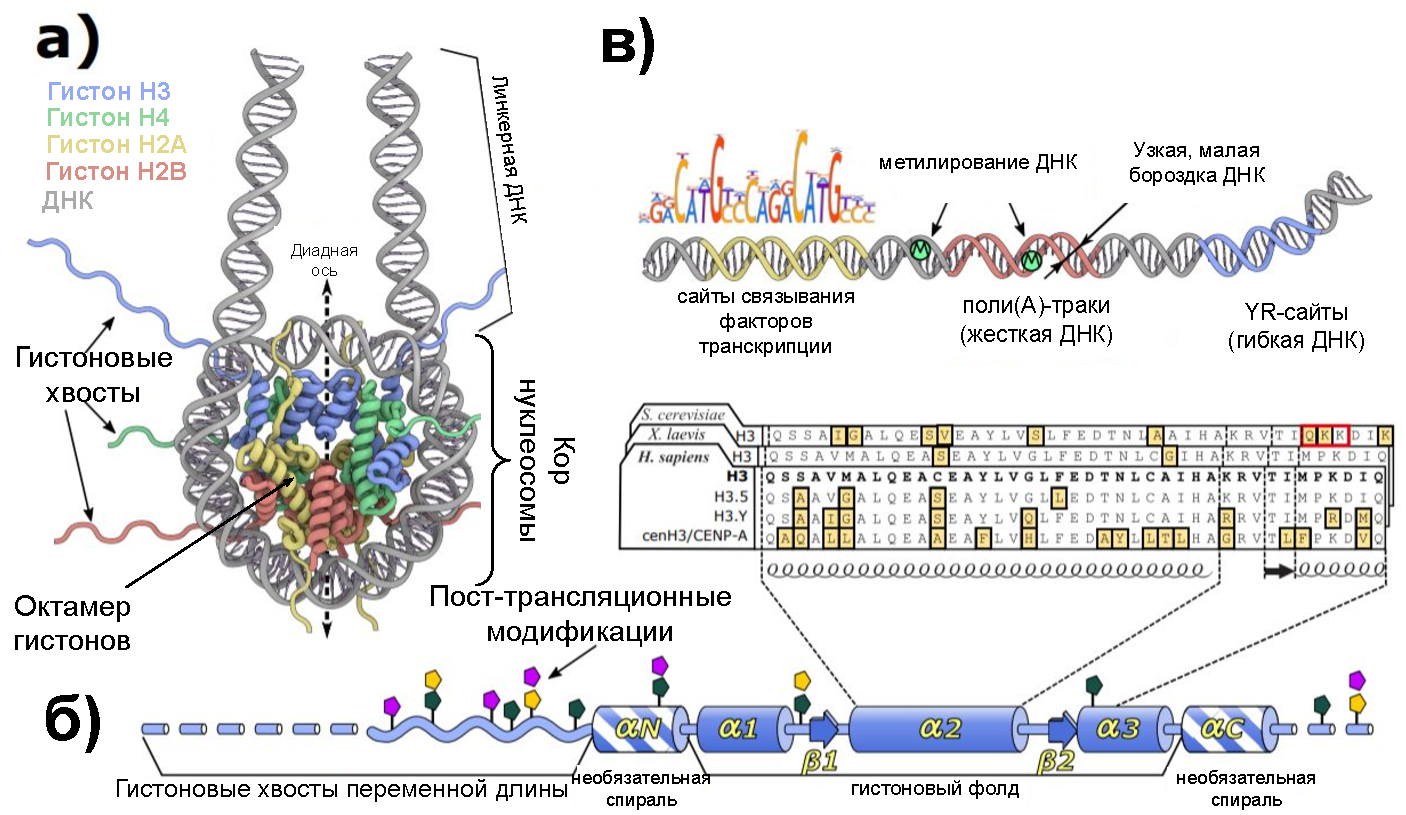
\includegraphics [width=\textwidth]{images/p2/cosb/part2_1_f1.pdf}
    \caption[Структура и вариабельность нуклеосомы]{(a) Структура нуклеосомы состоит из коровой частицы нуклеосомы (NCP), фланкированной линкерными сегментами ДНК. Коровая частица образована октамером гистонов, вокруг которого обернуты 145–147 пар оснований ДНК в виде левой суперспирали. Октамер состоит из двух пар гетеродимеров гистонов (H3-H4 и H2A-H2B) и обладает осью псевдосимметрии второго порядка (диадной осью), проходящей через центральную пару оснований нуклеосомной ДНК (диаду). Неструктурированные гистоновые хвосты отходят от глобулярной части белков. Малая бороздка ДНК обращена к октамеру гистонов в 14 специально предназначенных для этого сайтах связывания (в каждом сайте связывания боковая цепь остатка аргинина вставлена в малую бороздку). 
    (б) Схема типичной структуры гистонового белка: гистоновый фолд (спирали $\alpha$1, $\alpha$2 и $\alpha$3, листы $\beta$1 и $\beta$2) с необязательными спиралями $\alpha$N, $\alpha$C и гистоновыми хвостами переменной длины. Гистоновые ПТМ могут располагаться по всей длине белка и играть важную роль в функционировании хроматина, обеспечивая эпигенетическую разметку. Вариации гистонового сиквенса существуют как между организмами, так и внутри организма (гистоновые варианты).
    (в) ДНК - ключевой компонент нуклеосомы. Конкретные последовательности ДНК могут обеспечивать присутствие сайтов связывания факторов транскрипции в областях нуклеосомной ДНК, повышенную жесткость и/или изменения геометрии ДНК.}
    \label{fig:part2_1_f1}
\end{figure}



\subsection{Обзор динамических мод нуклеосом}

    Внимание на динамическую природу нуклеосом впервые было обращено в контексте отворачивания ДНК от октамера гистонов \cite{polach_mechanism_1995} (Рис. \ref{fig:part2_1_f2}a, в центре). Результаты экспериментов по ферментативному расщеплению ДНК \cite{polach_mechanism_1995}, измерению FRET \cite{li_nucleosomes_2004}, крио-ЭМ \cite{bilokapic_histone_2018} свидетельствуют о возможности откручивания ДНК (иногда называемом раскручиванием или дыханием ДНК). Данные процесс важен для доступа факторов транскрипции \cite{zaret_pioneer_2016,li_nucleosomes_2004} и РНК-полимераз \cite{bondarenko_nucleosomes_2006} к последовательности ДНК. Позднее выяснилось, что откручивание ДНК может происходить вместе с раскрытием димера H2A-H2B (состояние ``бабочка'') \cite{bohm_nucleosome_2011} или его полной диссоциацией (с образованием гексасомы), что часто происходит при транскрипции \cite{kireeva_nucleosome_2002}. Частично собранные нуклеосомы (также называемые субнуклеосомными структурами), такие как тетрасома или гемисома (полунуклеосома) также эффективно способствуют отворачиванию ДНК \cite{rychkov_partially_2017}. Недавно с использованием метода ChIP-exo было показано, что такие структуры широко распространены в динамическом хроматине в масштабе всего генома  \cite{rhee_subnucleosomal_2014}. В то время как тетрасомы могут возникнуть из-за потери двух димеров H2A-H2B нуклеосомой, динамические пути, ведущие к гемисомам, не совсем ясны. Новые экспериментальные данные подтверждают идею о том, что сборка нуклеосом \textit{in vivo} во время репликации ДНК происходит через депонирование тетрамеров H3-H4 (два димера H3-H4, взаимодействующие через четырехспиральную связку) с помощью фактора сборки хроматина 1 (CAF1) \cite{sauer_insights_2017,mattiroli_dna-mediated_2017}. После этого к ним присоединяются димеры H2A-H2B. Следовательно, маловероятно, что гемисомы образуются во время регулярной сборки нуклеосом. Расщепление нуклеосом на полунуклеосомы во время транскрипции - еще одна гипотеза (рассмотренная в \cite{zlatanova_nucleosome_2009}). Хотя есть некоторые споры, частным случаем статической структуры полунуклеосом могут быть центромерные нуклеосомы \textit{S. cerevisiae} \cite{henikoff_remarkable_2017}, которые также могут быть воссозданы \textit{in vitro} в особых условиях \cite{furuyama_reconstitution_2013}. В то время как нуклеосома в отсутствие внешнего сверхспирального стресса содержит ДНК в виде левосторонней суперспирали \cite{bancaud_structural_2006}, тетрасомы или гемисомы демонстрируют повышенную тенденцию к адаптации правостороннего состояния. Вероятно, так обстоит дело с центромерными нуклеосомами пекарских дрожжей [\textit{ibid.}] и тетрамерами гистонов архей \cite{marc_archaeal_2002}.



    В левой части рисунка \ref{fig:part2_1_f2} мы сгруппировали динамические режимы с меньшей величиной конформационных изменений (``компактная нуклеосома''), которые, тем не менее, функционально важны. Октамер гистона способен к ``расщеплению'' - изменению расстояния между двумя половинками нуклеосомы вдоль оси суперспирали ДНК. Экспериментально это наблюдалось на  нуклеосомах \cite{ngo_nucleosomes_2015,falk_cenp-c_2015} и может быть связано со скольжением витков ДНК относительно друг друга \cite{falk_cenp-c_2016}. Недавно наше понимание динамики октамера было дополнительно расширено за счет концепции пластичности октамеров на уровне отдельных димеров гистонов - точечные сшивки внутри димера H3-H4 ограничивает его деформируемость и ингибируют передвижение нуклеосом ремоделером SNF2h \cite{sinha_distortion_2017}. Наконец, ДНК в нуклеосоме - это компонент, который проявляет конформационную изменчивость. Октамер может скользить по ДНК, изменяя ротационное и трансляционное позиционирование ДНК \cite{shaytan_hydroxyl-radical_2017,shaytan_structural_2018}. Этот процесс сильно зависит от последовательности ДНК (обзор см. в \cite{eslami-mossallam_nucleosome_2016}) и включает локальные деформации ДНК, такие как дефекты скручивания \cite{edayathumangalam_nucleosomes_2005}. В линкерной области ДНК более гибкая, чем остальная часть ДНК \cite{gansen_structural_2009}. Благодаря такой высокой мобильности, комплексы нуклеосом с линкерным гистоном могут образовывать ансамбль различных конфигурации (см. обзор в \cite{ozturk_toward_2018}).


\begin{figure} [H]
    \centering
    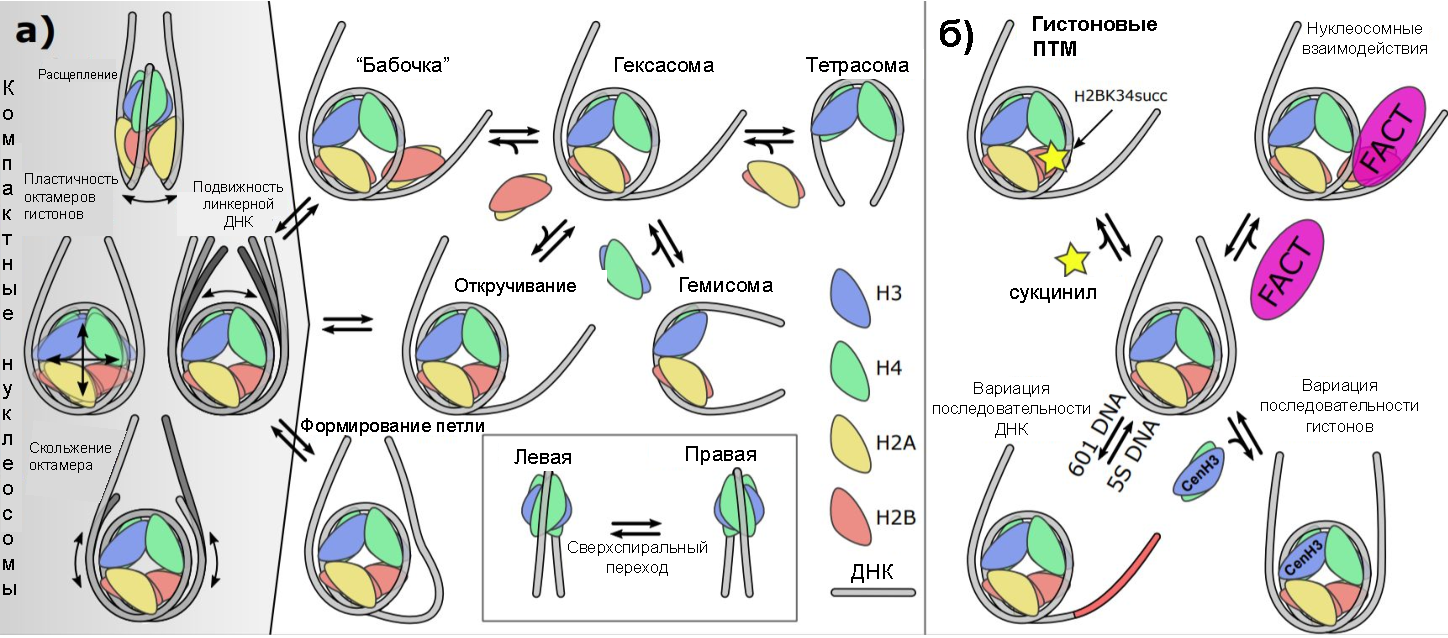
\includegraphics [width=\textwidth]{images/p2/cosb/part2_1_f2.pdf}
    \caption[Моды динамики нуклеосом]{(а) Обзор различных мод динамики нуклеосом. Слева (серая область) показаны режимы, сохраняющие компактность нуклеосомы. Справа показаны моды с большей амплитудой: нуклеосомная ДНК может спонтанно образовывать петли или отворачиваться от гистонов; большие состояния разворачивания ДНК способствуют образованию субнуклеосомных частиц: гексасом, тетрасом, гемисом.
    (б) Примеры факторов, влияющих на структурную динамику нуклеосом. Слева вверху: сукцинилирование H2B по лизину 34 способствует разворачиванию ДНК \cite{jing_site-specific_2018}. Справа вверху: ассоциация с фактором транскрипции FACT изменяет динамику развертывания нуклеосом \cite{valieva_large-scale_2016}. Слева внизу: разные последовательности ДНК имеют разную динамику разворачивания \cite{mauney_local_2018}. Справа внизу: вариант гистона H3 человека CENP-A изменяет подвижность линкерной ДНК \cite{roulland_flexible_2016}.}
    \label{fig:part2_1_f2}
\end{figure}


\subsection{Факторы, влияющие на динамику нуклеосом: недавние примеры}

    Факторы, влияющие на динамику нуклеосом можно разделить на четыре группы (Рис. \ref{fig:part2_1_f2}б): вариации последовательностей гистонов, вариации последовательности ДНК, ПТМ гистонов и различные белки, взаимодействующие с нуклеосомами.

     Белки, взаимодействующие с  нуклеосомами, включают в себя структурные белки хроматина (включая линкер гистона H1 \cite{lyubitelev_structure_2016}), шапероны гистонов, факторы транскрипции (включая пионерские факторы транскрипции \cite{zaret_pioneer_2016}), компоненты репликационного, транскрипционного и эпигенетического аппарата. Они могут влиять на любой из обсуждаемых режимов динамики нуклеосом. Например, гистоновый шаперон FACT обратимо разворачивает нуклеосомную ДНК с обоих концов \cite{valieva_large-scale_2016}, чтобы облегчить обмен димера гистона H2A-H2B \cite{wang_histone_2018}. Гистоновый шаперон Nap-1 является другим примером, он вытесняет димер H2A-H2B из нуклеосомы, и может действовать без необходимости изначального отворачивания ДНК \cite{lee_single-molecule_2017}. Показано, что на раскрытие центромерных нуклеосом влияет взаимодействие с белком CENP-C \cite{falk_cenp-c_2015}. Напротив, ПАРП-1 (многодоменный белок, который управляет обнаружением одно- и двухцепочечных разрывов во время репарации ДНК) значительно увеличивает расстояние между супервитками нуклеосомной ДНК в обратимой манере \cite{sultanov_unfolding_2017}. Линкерные участки ДНК могут притягиваться друг к другу гистоном H1, который снижает их гибкость \cite{bednar_structure_2017}.

    Неструктурированные гистоновые хвосты исторически были основными целями для исследования эффектов различных PTM гистонов на динамику нуклеосом \cite{bowman_post-translational_2015} (Рис. \ref{fig:part2_1_f1}б). По умолчанию считается, что модификации, изменяющие заряд (например, ацетилирование лизина, фосфорилирование серина или отщепление гистонового хвоста), вызывают дестабилизацию нуклеосом за счет снижения не-специфического электростатического притяжения между ДНК и гистонами \cite{fenley_modulation_2018}. Однако существуют свидетельства в пользу того, что более тонкие эффекты также могут иметь значение, такие как изменения вторичной структуры гистоновых хвостов (напр., для H4K16ac \cite{potoyan_regulation_2012}). ПТМ, расположенные на сайтах связывания гистонов с ДНК, могут оказывать более специфические эффекты, нарушая связывание с ДНК соответствующих местах. Например, недавно проанализированное сукцинилирование H2BK34, расположенного в сайте связывания ДНК гистонами на расстоянии $\sim$25 п.н. от точки входа/выхода в нуклеосоме, ингибирует сборку нуклеосом и способствует разворачиванию ДНК \cite{jing_site-specific_2018}. Важность ПТМ гистонов, локализованных в глобулярной части гистонов, и их функциональное значение в настоящее время также широко признаны. Например, H3K56ac облегчает разворачивание нуклеосом и играет важную роль в регуляции сборки нуклеосом \cite{zhang_multisite_2018}. Не изменяющие заряд ПТМ, такие как H3R42me2, также могут способствовать дестабилизации нуклеосом \cite{casadio_h3r42me2a_2013}; последний также использовался микобактериями для изменения эпигенетического ответа хозяина \cite{yaseen_mycobacteria_2015}. ПТМ на границах раздела гистон-гистон могут как нарушать образование октамера \cite{ye_histone_2005}, так и стабилизировать нуклеосомы (например, H4K77ac из-за устранения электростатического отталкивания внутри димера гистона \cite{fenley_modulation_2018}). Сходным образом, H1K85ac ведет к общей стабилизации хроматина и линкерной ДНК за счет увеличения связывания глобулярного домена H1 с коровыми гистонами \cite{li_histone_2018}.

    Нет сомнений в том, что вариация последовательности ДНК может оказывать значительное функциональное воздействие, изменяя вероятность разворачивания ДНК и стабильность нуклеосом. Например, сильно взаимодействующая последовательность ``601'', если ее поместить на нуклеосому, образует полярный барьер для транскрипции \cite{bondarenko_nucleosomes_2006}. Это соответствует известному асимметричному разворачиванию последовательности ``601'' под напряжением \cite{ngo_asymmetric_2015} и в состоянии покоя. Последнее было недавно подтверждено малоугловым рассеянием рентгеновских лучей по сравнению с симметричным разворачиванием, наблюдаемым для 5S рибосомной последовательности \cite{mauney_local_2018}. Динамические эффекты также играют роль во время связывания факторов транскрипции, как первоначально было предложено J. Widom и соавторами \cite{polach_mechanism_1995}. Например, недавняя крио-ЭМ структура нуклеосомы, включающая энхансерную последовательность ALB1 (ALB1 является сайтом связывания для пионерского фактора транскрипции FoxA), аналогична структуре 601-нуклеосомы, но ДНК в области связывания FoxA является более подвижной, способствующей связыванию FoxA \cite{takizawa_cryo-em_2018}. Несмотря на многочисленные усилия, точная взаимосвязь между последовательностью ДНК и ее влиянием на динамику нуклеосом все еще не ясна. По данным некоторых работ присутствие гибких пиримидин-пуриновых динуклеотидов (YR) в сайтах связывания ДНК является важным фактором для позиционирования ДНК и силы связывания (Рис. \ref{fig:part2_1_f1}в) \cite{cui_structure-based_2010,segal_dna_2009}. Однако развитию более общих теоретических моделей в настоящее время препятствует отсутствие достаточно подробных и воспроизводимых экспериментальных наборов данных о связи последовательности ДНК с ее стабильностью на нуклеосоме \cite{eslami-mossallam_nucleosome_2016}. Атомистическое и крупнозернистое компьютерное моделирование может восполнить этот пробел: как недавно показали несколько исследований с использованием моделирования, в зависимости от физических свойств последовательности ДНК, ее транслокация может предпочтительно происходить через винтовой механизм ``распространения дефектов кручения'' или механизм ``повторного захвата петли'' \cite{lequieu_silico_2017,niina_sequence-dependent_2017}.

    Варианты гистонов обеспечивают богатый репертуар вариаций канонической гистоновой последовательности, варьирующийся от всего лишь нескольких аминокислотных различий (например, H3 vs H3.5) до довольно существенных различий, которые могут изменять несколько динамических режимов одновременно (Рис. \ref{fig:part2_1_f1}б). Напр., CENP-A (вариант, критический для образования центромер во время митоза) имеет более короткую спираль $\alpha$N, чем канонический H3. Эта особенность делает линкерную ДНК в CENP-A нуклеосомах более гибкой и влияет на связывание ДНК с гистонами \cite{roulland_flexible_2016}. Кроме того, CENP-A влияет на разворачивание ДНК и способствует образованию петель \cite{stumme-diers_nanoscale_2018}. Известно также, что нуклеосомы CENP-A демонстрируют расщепление половинок нуклеосомы вдоль оси суперспирали \cite{falk_cenp-c_2015}. Варианты с небольшими изменениями канонической гистоновой последовательности также могут быть функционально очень важными: H3.3 важен для пластичности нейронов \cite{maze_critical_2015}, H3.5 для сперматогенеза \cite{urahama_histone_2016}, а H3.Y изменяет регуляцию клеточного цикла \cite{wiedemann_identification_2010}. В последние годы было показано, что эти небольшие вариации последовательности могут влиять на стабильность и динамику нуклеосом. Например, H3.5-специфический остаток лейцина 103 дестабилизирует нуклеосому, что важно для процесса транскрипции в тестикулярных клетках человека \cite{urahama_histone_2016}. Как показано в \cite{kujirai_identification_2017}, в H3.Y метионин 124 способствует стабильной ассоциации тетрамера H3.Y-H4 с ДНК. Другой H3.Y-специфический остаток -- лизин 42 -- играет роль в придании гибкости линкерной ДНК. 
    
    Более того, оказывается, что небольшие вариации между последовательностями канонических гистонов, кодируемых разными копиями генов канонических гистонов у человека, также могут функционально влиять на стабильность нуклеосом. Вариации M51L и K99R в гене гистона HIST1H2AH (изоформа H2A1H) приводят к стабилизации нуклеосом и изменяют пролиферацию клеток \cite{bhattacharya_histone_2017}. Точно так же теперь описаны эффекты небольших вариаций между каноническими последовательностями у разных видов. Специфичный для грибов гистоновый мотив H3 QKK (Рис. \ref{fig:part2_1_f1}в), расположенный на оси диады нуклеосомы, вносит вклад в плохую сборку октамеров в нуклеосомах дрожжей \cite{leung_unique_2016}.


\subsection{Тонкие детали динамики нуклеосом}

    Если распечатать димеры гистонов на 3D-принтере то из можно собрать в октамера подобно конструктору LEGO (см. 3D-печатные модели нуклеосом на \url{https://github.com/intbio/nuclLEGO}). Этот взгляд на нуклеосому как на жесткую модульную структуру теперь уступает место альтернативному взгляду на нуклеосому как на динамическую сущность, где даже небольшие конформационные вариации функционально важны. В поддержку последней точки зрения мы обсудим несколько недавних наблюдений, представленных на рисунке \ref{fig:part2_1_f3}. Во-первых, динамика ДНК внутри нуклеосомы выходит за рамки простого разворачивания и может демонстрировать различные искаженные конформации, включая дефекты кручение и выпячивание ДНК вблизи точки входа/выхода. Такого рода изменения недавно наблюдались как при атомистическом моделировании \cite{shaytan_coupling_2016} (Рис. \ref{fig:part2_1_f3} a), так и на крио-ЭМ картах \cite{bilokapic_histone_2018} (Рис.\ref{fig:part2_1_f3}в). Более того, изменения в конформации ДНК связаны с тонкими изменениями конформации гистоновых белков. Например, как показано в крио-ЭМ, разворачивание 15 пар оснований ДНК с одной стороны октамера гистонов приводит к изменениям конформации гистонов вблизи точек входа / выхода с обеих сторон, а также сопровождается общим небольшим расширением октамера перпендикулярно оси симметрии нуклеосомы \cite{bilokapic_histone_2018}. Более того, определенная связь между перестройками гистонового ядра и конформацией ДНК также наблюдалась для полностью завернутого состояния (Рис.\ref{fig:part2_1_f3}г), было показано, что нуклеосомы могут сокращаться на 8\% вдоль оси диады и расширяться на 5\% в перпендикулярном направлении \cite{bilokapic_structural_2018}.

  Пластичность индивидуальных димеров гистонов также функционально важна. В дополнение к недавно продемонстрированной важности пластичности H3-H4 для ремоделирования нуклеосом \cite{sinha_distortion_2017}, с помощью твердотельного ЯМР было показано, что внутренняя динамика во временных масштабах от наносекунд до миллисекунд присутствует для гистона H4 в нуклеосомах \cite{shi_structure_2018}. Недавнее исследование метил-TROSY ЯМР показало, что мутантные нуклеосомы могут проявлять значительно повышенную динамику внутри гистонов H3-H4 \cite{kitevski-leblanc_investigating_2018}. Помимо H3-H4, пластичность H2A-H2B, по-видимому, также имеет решающее значение для сборки и функционирования нуклеосом. В частности, сборка нуклеосом \textit{in vitro} со сшитыми димерами H2A-H2B происходит только до стадии гексасом \cite{bilokapic_histone_2018}, а это означает, что для сборки требуется определенная гибкость димера. Структура ЯМР  изолированного димера H2A-H2B в растворе, вероятно, отражает эти динамические режимы и демонстрирует повышенную гибкость и беспорядок, в частности, внутри дополнительных спиралей $\alpha$C и $\alpha$N по сравнению со структурой внутри нуклеосомы (Рис.\ref{fig:part2_1_f3}е) \cite{moriwaki_solution_2016}. Динамика H2A-H2B также, вероятно, используется ремоделером SWR1. Он распознает специфически канонические нуклеосомы, содержащие H2A, и заменяет H2A его вариантом H2A.Z. Способность ремоделера SWR1 распознавать и действовать на нуклеосомы H2A на не на H2A.Z недавно была связана с отличием нескольких аминокислот между H2A и H2A.Z. Причем ни одна из этих аминокислот не экспонируется на поверхности нуклеосом \cite{ranjan_h2a_2015}. Поскольку рентгеновские исследования показывают очень похожую структуру нуклеосом H2A и H2A.Z \cite{suto_crystal_2000}, эти открытия подразумевают, что присутствует некая динамическая сигнатура, которая используется для распознавания нуклеосом H2A.
    
    Наконец, тонкая динамика гибких гистоновых хвостов с их способностью взаимодействовать с ДНК и другими белками формирует еще один уровень динамической сложности. Гистоновые хвосты и другие белки хроматина несут положительно заряженные остатки (особенно аргинины \cite{west_electrostatic_2010,dragan_energetics_2003}), которые предпочитают взаимодействовать с малыми бороздками ДНК как участками отрицательного электростатического потенциала (Рис. \ref{fig:part2_1_f3} б). Эти взаимодействия могут, в свою очередь, модулироваться ПТМ гистонов или AT-богатыми последовательности ДНК (что способствует образованию узких малых бороздок \cite{freeman_dna_2014} и может распознаваться некоторыми белками в контексте нуклеосом \cite{xiao_molecular_2017}) (Рис. \ref{fig:part2_1_f1} в). 



\begin{figure} [H]
    \centering
    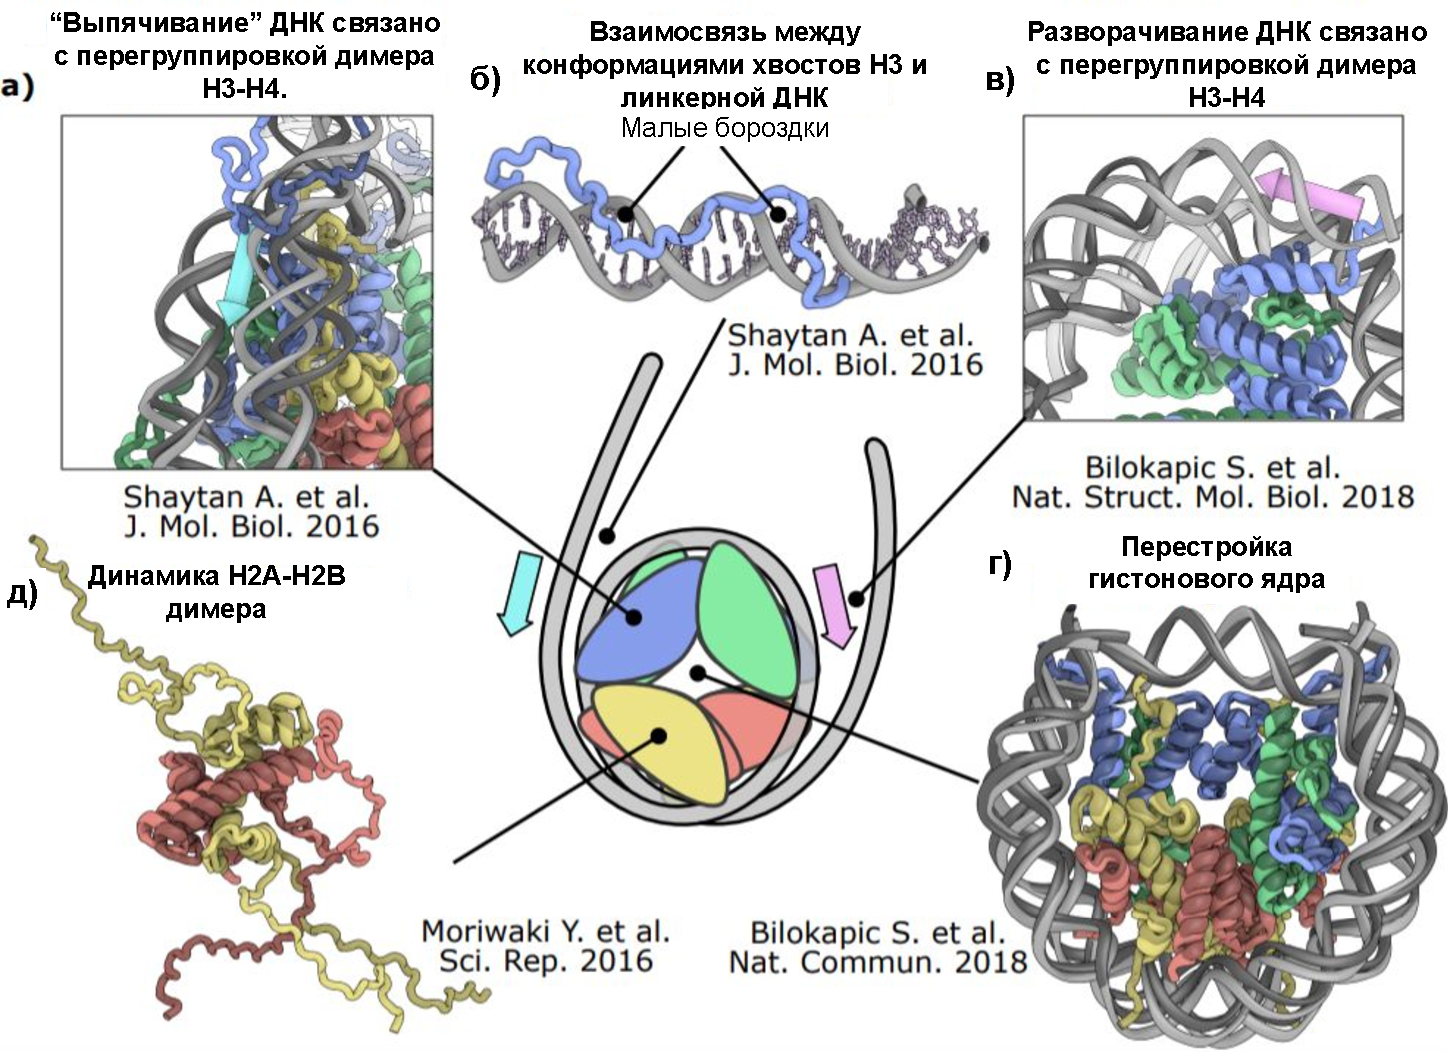
\includegraphics [width=\textwidth]{images/p2/cosb/part2_1_f3.pdf}
    \caption[Тонкие детали динамики нуклеосом]{Динамика ДНК в нуклеосомах тесно связана с динамикой гистонов (a, б, в, г). Цветовая схема соответствует рисунку \ref{fig:part2_1_f1}. Голубые и фиолетовые стрелки на центральной диаграмме и панелях (а) и (в) обозначают одни и те же области входа / выхода ДНК в нуклеосому. (а) Помимо простого разворачивания ДНК, ДНК может проявлять выпуклости возле точек входа / выхода, как это наблюдается в моделировании МД и крио-ЭМ \cite{bilokapic_histone_2018,shaytan_coupling_2016}.  (б) Гистоновый хвост H3 взаимодействует с линкерным сегментом ДНК. Наблюдаются преимущественные взаимодействия с малыми бороздками ДНК \cite{shaytan_coupling_2016}.
    (в) Раскручивание ДНК  сопровождается перестройками в димере гистона H3-H4 \cite{bilokapic_histone_2018}. Кристаллическая структура нуклеосомы показана светлыми цветами. 
    (г) Гистоновый октамер с полностью обернутой ДНК может принимать сжатую конформацию вдоль оси диады (темные цвета) по сравнению с кристаллической структурой по умолчанию (светлые цвета) \cite{bilokapic_structural_2018}. 
    (д) Гибкость димера гистона H2A-H2B, наблюдаемая с помощью ЯМР-исследований в растворе \cite{moriwaki_solution_2016}. Две конформации показаны темным и светлым цветами.}
    \label{fig:part2_1_f3}
\end{figure}














